\chapter{Konsept i Statistikk}

Dette kapittelet inneheld forklaringar til konsept i statistikk som ikkje er pensum i seg sjølv men som hjelper å løfte forståinga av det som er pensum. Konsepta i dette kapittelet er grunnleggande konsept for moderne statistikk og sannsynlegheitsteori.

\section{Friheitsgrad}\label{chap:friheitsgrad}
Antalet friheitsgrader er antalet verdiar i kalkulasjonen av ein statistikk (varians, gjennomsnitt, o.l) som er fri til å variere.

Det enklaste eksempelet er f.eks sjå for deg at vi har eit sett med observasjonar 

\begin{equation*}
    \{ 6, 8, 5, 9, 6, 8, 4, 11, 7, x \}
\end{equation*}

pluss informasjonen at $\sum X = 69 \implies \bar{X}=6.9$. Der X er observasjonen vi ikkje kjenner. Kva er friheitsgraden til denne ukjente $x$? På grunn av informasjonen i summen og/eller gjennomsnittet har $x$ ingen friheit til å variere siden $x$ nødvendigvis må vere $5$ i dette tilfellet. Dette er grunnen til at når ein nytter seg av gjennomsnittet til å rekne ut ein annan statistikk så minkar friheitsgraden, for eksempel i formelen for utvalgsvarians $S^2$:

\begin{equation*}
    S^2 = \frac{1}{n - 1} \sum_{i=1}^{n}(X_i - \bar{X})
\end{equation*}

Ein intuitiv og uformell måte å tenke på dette er at friheitsgrad er eit mål på usikkerheit og når vi får informasjon (f.eks gjennom gjennomsnittet) så blir usikkerheiten mindre. Friheitsgrad er eit viktig konsept i statistikk siden det er avgjerande for å få rette estimat og for å rette p-verdiar i hypotesetestar.

\section{Sentralgrenseteoremet}\label{chap:sentralgrense}

Sentralgrenseteoremet fortel oss at summen / gjennomsnittet av uavhengige stokastiske variablar $X$ er normalfordelt sjølv om den underliggande fordelingen til $X$ ikkje er normalfordelt. Meir formelt, om me har $n$ utvalg frå $X$ med ukjent fordeling med forventingsverdi $\mu$ og varians $\sigma^2$ så vil den stokastiske variabelen

\begin{equation}
    Z = \frac{\bar{X} - \mu}{\sigma / \sqrt{n}} \sim N(z; 0, 1)
\end{equation}

når $n \rightarrow \infty$. For å visualisere. Sjå på figur \ref{fig:CLT}. Der ser me at $\bar{X}$ for veldig forskjellige fordelingar av $X$ vil vere normalfordelt. Dette er eit veldig viktig konsept sidan det innebærer at mange problem der den underliggande fordelinga ikkje er normalfordelt kan løysast ved hjelp av normalfordelinga.

\begin{figure}[H]
    \centering
    \label{fig:CLT}
    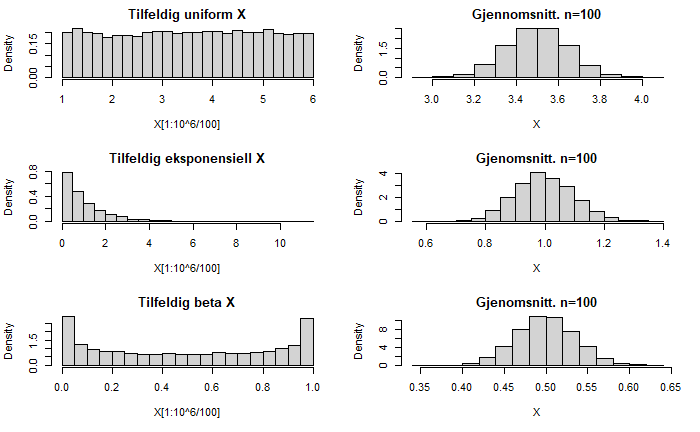
\includegraphics[width=\textwidth]{bilete/CLT.png}
    \caption{Demonstrasjon av sentralgrenseteoremet. Til venstre har me 1000 utvalg frå forskjellige fordelingar, høvevis uniform, eksponensiell og beta. Til høgre har me 1000 utvalg av gjennomsnittet til 100 verdier frå høvevis uniform eksponensiell og betafordelingen.}
\end{figure}